
\section{PSR J1119$-$6127: Characterization a High Magnetic Field Pulsar with Single-Altitude Model}

\paperref{This section is based on work done for
``Observations of Energetic High Magnetic Field Pulsars with the
\it{Fermi} Large Area Telescope'' \citep{parent2011observations}.}

\begin{figure}[t!!]
%\begin{center}
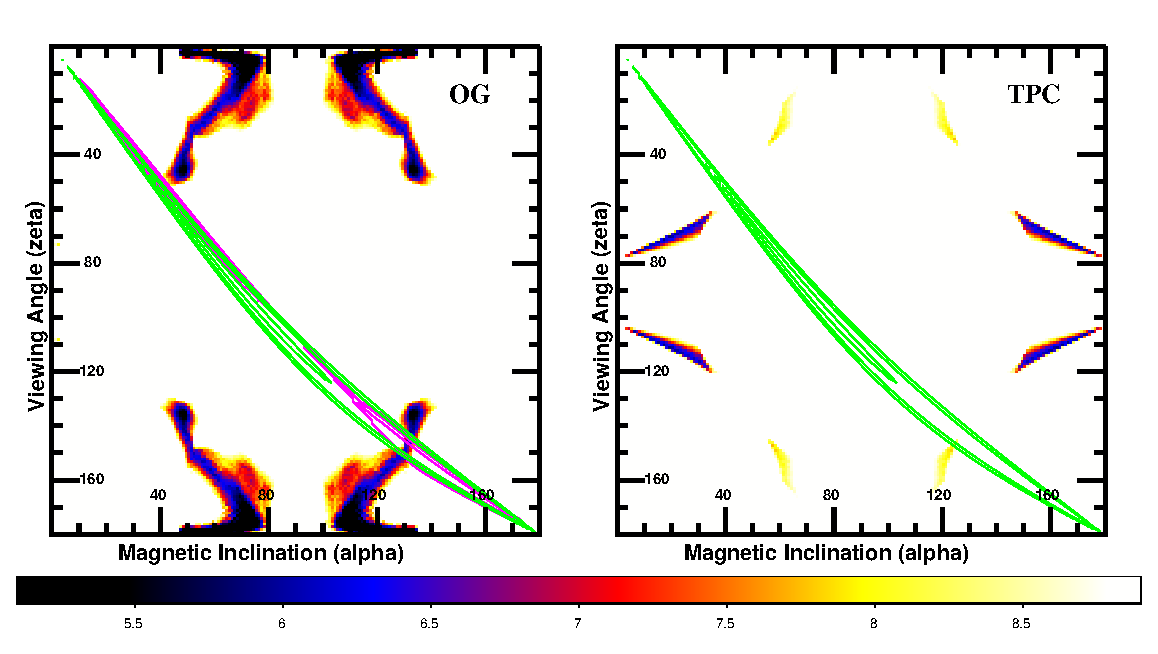
\includegraphics[width=0.99\textwidth]{chapters/multiWaveLength/figures/HBP_fig3_rev.eps}
\caption[Pulsar geometry and emission modeling fit map for PSR~J1119$-$6127 with the outer gap
(left panel) and the two-pole caustic (right panel) models in the $\alpha$--$\zeta$ plane]{
Figure taken from \cite{parent2011observations}.
Pulsar geometry and emission modeling fit map for PSR~J1119$-$6127 with the outer gap
(left panel) and the two-pole caustic (right panel) models in the $\alpha$--$\zeta$ plane. Green contours show
the RVM fit to the \cite{weltevrede2011glitch} radio polarization data. For
the left panel we also show the polarization fit for finite-altitude, open zone
radio emission ($R=0.09\,R_{\rm{LC}}$, magenta contours). Contours are at
1.5, 2.5, and 3.5 times the minimum value of the reduced
$\chi^2 = 0.85$. The background color scale gives the $\chi_3$ statistic fit to
the observed $> 500$\,MeV $\gamma$-ray pulse profile. The color scales in the panels are the
same, with dark colors representing better fits. Preferred models lie along the
diagonal polarization fit band. \label{fig:roger_goodness}}
%\end{center}
\end{figure}

\begin{figure}
\begin{center}
\includegraphics[scale=0.75]{chapters/multiWaveLength/figures/HBP_fig4_rev.eps}
\caption[Light curves and radio polarization of PSR~J1119$-$6127 overlaid with models]{
Figure taken from \cite{parent2011observations}.
Light curves and polarization of PSR~J1119$-$6127 overlaid with models. The bottom panel shows the Parkes
radio light curve in the two peaked (post-glitch) mode, which provides the best
model constraints. The corresponding radio polarization position angle data are
shown (right scale) in the upper panel. The model pulsar phase ($\phi_{\rm{B}}$, bottom axis) is
referenced to the closest approach of the magnetic axis to the Earth
line-of-sight, as fit from the polarization sweep. The sweep rate maximum
(green arrow) and pulse profile offsets (magenta arrow) are shown, with good
matches to the observed radio data for an altitude of $R=0.09 R_{\rm{LC}}$. The
upper panel shows the {\it Fermi} pulse profile (left scale) and model outer gap (solid line)
and two-pole caustic (dashed line) profiles. These are best-fit profiles (geometric angles
in the legend) and the phase is referenced to the radio-determined phase of the
magnetic axis. The $\gamma$-ray background, shown by the dotted line, was
estimated using an annular ring centered on the radio position with inner and
outer radii of 0.5\degr\ and 1.5\degr\ respectively, during the off-pulse
region. \label{fig:roger_lcs} } \end{center}
\end{figure}

In the paper \cite{parent2011observations}, detection 
with the {\it Fermi} Large Area Telescope
of PSR J1119-6127 (Period $=0.408s$) and 
upper limits of pulsars PSR J1718-3718, PSR J1734-3333 and PSR J1846-0258
are reported and criteria for non-detection are discussed.
These pulsars have high magnetic fields.
In the paper, the spectrum of PSR J1119-6127 is concluded to be more 
similar to a young pulsar rather than a magnetar as might
be expected from such a high magnetic field.

Data used to analyze the radio polarization was
taken during a 
glitch recovery in PSR J1119-6127 wherein
more data per phase was available.
Because of the larger number of avaliable data points,
modeling the polarization position
angles was more constraining.
Data analysis details are given in 
\cite{weltevrede2010pulsar} and \cite{hobbs2004long}.

In the $\gamma$-ray modeling, both two-pole caustic
and outer gap models were tested with
$w=0.02$.  Results of these fittings are seen in 
Figure~\ref{fig:roger_goodness}. 
The figure of merit here is the  
$\chi_3$ weighting defined in \cite{romani2010constraining}.
Additionally, on the plot are the  
RVM fit contour results in green as well as a numerical 
single-altitude model fit contour in magenta.  
Two-pole caustic fitting results and the polarization
fitting results have poor overlap compared to the outer gap model.
The best models are at $\alpha=125^\circ$ to $130^\circ$
and $\zeta=140^\circ$ to $150^\circ$ for the outer
gap model and at $\alpha=125^\circ$ and $\zeta=145^\circ$
for the two-pole caustic model. 
The two models give similar geometry angles but 
the outer gap model is a better
fit over a larger parameter space as can be seen in Figure~\ref{fig:roger_lcs}

The best fit parameters for polarization
modeling yield reduced $\chi^2$ of 1.1
The altitude of emission derived
from polarization fitting is $0.1R_{\rm{LC}}$.
It is interesting to note that 
using the BCW model yields lower altitudes 
\citep{weltevrede2011glitch} and requires smaller
$\alpha$ for emission originating in the open zone.



